\section{Empirical grounding in public data}
\label{sec:grounding}

Three questions decide whether the design is sound. Does the website's blink detector count blinks correctly? Do the signals BlinkTwin measures move with sleepiness? And is the link between objective signals and subjective sleepiness similar enough across people that one population mapping would do? We used two public datasets to answer them and to set the population mappings of the twin.

\subsection{DROZY: three sessions of increasing sleep deprivation}
\paragraph{Data.} DROZY \citep{massoz2016ulg} contains 14 adults who each performed three 10-minute PVTs over a period of increasing sleep deprivation. For each test it provides the KSS rating, the stimulus and response times of the PVT, near-infrared face video from a Kinect sensor at 30 frames per second (15 for some tests), 68 facial landmarks for every frame, and polysomnographic signals including the vertical electro-oculogram (EOG). Five tests are missing and one did not take place, leaving 36 tests from 14 subjects (12 per test number). DROZY may be used for research only and may not be redistributed; no images from it are shown here, and only aggregate statistics are reported.

\paragraph{Methods.} For each test we computed the PVT median reaction time, the mean response speed and the number of lapses longer than 500~ms, the threshold for the standard 10-minute PVT \citep{basner2011maximizing}. For the eyes we ran the website's blink meter (Section~\ref{sec:system}) unchanged on the landmarks (\texttt{web/scripts/drozy\_eyes.ts}). The website feeds it MediaPipe's eye-closure blendshape; here the equivalent closure score was the eye aspect ratio \citep{soukupova2016real} rescaled within each test between its 90th percentile (open) and 1st percentile (closed). As ground truth for blinks we detected positive deflections in the vertical EOG, band-passed at 0.5--15~Hz, with a prominence of at least 5 times the scaled median absolute deviation and a width of 40--600~ms (\texttt{analysis/drozy\_eog.py}). Associations with KSS were estimated with linear mixed models with a random intercept per subject and with repeated-measures correlations; models with random slopes did not converge and are not used. Code: \texttt{analysis/drozy\_analysis.py}.

\paragraph{Blink detection agrees with EOG.} Across the 36 tests, blink rates from the website's blink meter agreed with EOG blink rates (Spearman $\rho$ = 0.88, Pearson r = 0.89; Figure~\ref{fig:drozy-blink}). The meter counted 5.4 fewer blinks per minute than the EOG on average, with 95\% limits of agreement from $-19.1$ to $+8.3$ blinks per minute.

\paragraph{Signals move with sleepiness.} From the first to the third test, mean KSS rose from 3.25 to 5.58 to 7.33, median reaction time from 346 to 391 to 417~ms, lapses from 4.3 to 14.8 to 23.8, PERCLOS from 2.85\% to 4.48\% to 5.86\%, and mean blink duration from 180 to 225 to 243~ms. Blink rate stayed flat at about 31--32 per minute. In mixed models, KSS rose by 2.22 points per 100~ms of median reaction time (95\% CI 1.07 to 3.37, p = $1.5\times10^{-4}$), by 0.28 points per percentage point of PERCLOS (0.08 to 0.48, p = 0.006) and by 1.92 points per 100~ms of blink duration (0.71 to 3.14, p = 0.002); blink rate was not related to KSS (p = 0.55). Within-person (repeated-measures) correlations with KSS, with 21 degrees of freedom, were 0.77 for median reaction time, 0.73 for lapses, 0.53 for PERCLOS, 0.51 for blink duration and 0.35 for blink rate (not significant) (Figure~\ref{fig:drozy}).

\paragraph{Personal calibration did not help here.} We tested BlinkTwin's central idea directly. For each held-out subject, the first available test served as a calibration check-in and the later tests were predicted from median reaction time, with the population model fitted on the other subjects (leave one subject out, 22 predictions). The population model alone had a mean absolute error of 1.68 KSS points. Shifting the person's intercept fully to match the check-in gave 2.36, and shifting it by the shrinkage factor that BlinkTwin's Kalman update applies gave 1.90. Carrying the check-in rating forward gave 3.45, and predicting the population mean gave 2.04. For the 9 subjects with all three tests, using the first two tests as check-ins to predict the third gave 2.08 with the Bayesian update in Eq.~\eqref{eq:blr}, against 1.82 for the population model. The eye features behaved the same way. In DROZY, therefore, calibration from one or two check-ins did not improve on the population mapping. The reasons are plausible: the sample is small; the residual noise of a single KSS rating around the model (SD 1.57) is larger than the between-person spread of intercepts (SD 1.14), so one rating says little about the person; the third test extrapolates beyond the calibration range; and the reaction-time slope was similar across people (9 subjects with three tests; individual slopes 2.5 to 7.5 KSS points per 100~ms, all positive, with no between-person variance left after removing estimation noise). Personal calibration is therefore a hypothesis to be tested in the validation study; the simulation in Section~\ref{sec:simulation} shows the conditions in which it helps.

\paragraph{Population mappings for the twin.} The reaction-test mapping in Table~\ref{tab:params} is the random-intercept model above: intercept 3.494, slope 2.222 KSS points per 100~ms, prior SD of the intercept 1.136 (the between-subject SD), residual SD 1.572. The webcam mapping is a joint model of PERCLOS and blink duration (intercept 3.609, slopes 0.187 per percentage point and 1.441 per 100~ms, residual SD 1.896). The prior SDs of the slopes come from random-slope fits that did not converge and are used only as weakly informative values. The person-level distributions of the virtual participants in Section~\ref{sec:simulation} were also taken from DROZY.

\begin{figure}[t]
  \centering
  \includegraphics[width=\linewidth]{../results/fig_drozy.pdf}
  \caption{DROZY. KSS across the three tests, and KSS against PVT median reaction time and mean blink duration, one line per subject, with within-person correlations. Aggregate statistics only; no images.}
  \label{fig:drozy}
\end{figure}

\begin{figure}[t]
  \centering
  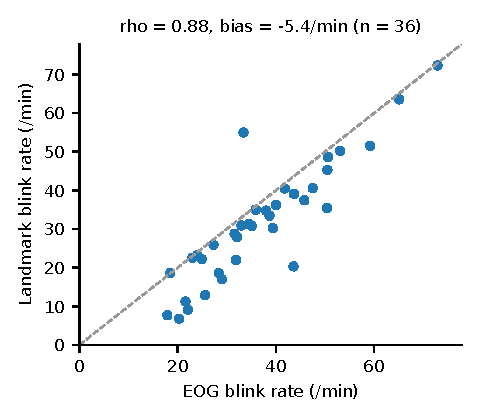
\includegraphics[width=0.48\linewidth]{../results/fig_drozy_blink_validation.pdf}
  \caption{Blink rate from the website's blink meter, run on DROZY landmarks, against blink rate from the vertical EOG, one point per test (n = 36).}
  \label{fig:drozy-blink}
\end{figure}

\subsection{OpenNeuro ds004902: normal sleep and sleep deprivation}
\paragraph{Data.} The dataset contains 71 adults, each tested once after a night of normal sleep and once after a night of sleep deprivation, in counterbalanced order \citep{xiang2024resting,xiang2024ds004902}. We used only the released participant table, which gives the number of PVT lapses, the median reaction time and its standard deviation, the KSS and the SSS for each session. In this release KSS and SSS were collected on different participants: only 2 people have KSS and SSS in both sessions, and only 2 have both KSS and PVT results in both sessions. PVT and SSS overlap for 25 people, so person-level coupling was analysed with the SSS.

\paragraph{Analysis.} Paired changes (sleep deprivation minus normal sleep) were tested with the Wilcoxon signed-rank test, with $d_z$ (mean change divided by the standard deviation of the change) as the effect size. Coupling between the change in median reaction time and the change in SSS was measured with Spearman's $\rho$. Code: \texttt{analysis/openneuro\_pvt\_kss.py}.

\paragraph{Results.} Sleep deprivation raised KSS by 2.03 points on average (SD of change 2.04; median 5 after normal sleep and 7 after sleep deprivation; n = 33, $d_z$ = 1.00, p = $5.1\times10^{-5}$) and SSS by 1.66 points (n = 35, $d_z$ = 0.80, p = $2.7\times10^{-4}$). Median reaction time slowed by 41.2~ms (SD of change 30.9~ms; median 320~ms after normal sleep and 359~ms after sleep deprivation; n = 30, $d_z$ = 1.33, p = $1.5\times10^{-5}$). The number of lapses did not change (mean change $-0.03$, n = 30, p = 0.92). Reaction time slowed in 90\% of participants, while KSS rose in 73\%. Across the 25 people with both measures, the change in reaction time was only weakly related to the change in SSS (Spearman $\rho$ = 0.25, p = 0.22; Pearson r = 0.37, p = 0.067) (Figure~\ref{fig:openneuro}).

\paragraph{Interpretation.} At the group level both signals respond strongly to sleep loss. For an individual, how much reaction time slowed says little about how much sleepier the person feels. This is the situation the per-channel bias of the twin is designed for: a passive channel may misread a person, and the person's own ratings should stay the reference. Two cautions apply: the sample is small, and with two sessions per person the change scores carry the measurement error of both sessions. The weak coupling across people in ds004902 and the uniform reaction-time slope in DROZY are not in conflict: the first concerns how much each person's state changed, the second how each person's KSS maps onto reaction time.

\begin{figure}[t]
  \centering
  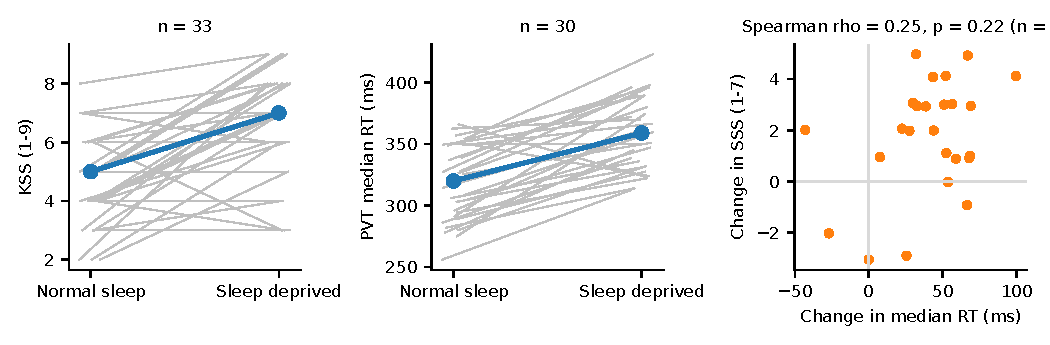
\includegraphics[width=\linewidth]{../results/fig_openneuro.pdf}
  \caption{OpenNeuro ds004902. Left and middle: KSS and PVT median reaction time after normal sleep and after sleep deprivation (grey: individuals; blue: medians). Right: change in median reaction time against change in SSS for the 25 people with both measures.}
  \label{fig:openneuro}
\end{figure}
